\documentclass{subfiles}

\begin{document}


    \begin{Frage}
        Kernspin, magnetisches Moment, gyromagnetisches Verhältnis.
    \end{Frage}
    \begin{Antwort}
        Unter dem \href{https://de.wikipedia.org/wiki/Kernspin}{\emph{Kernspin}} versteht man den Gesamtdrehimpuls $I$ eines Atomkernes um seinen Massenschwerpunkt $\mu(m)$. Dabei ist $m\in\R^N$ ein Tupel aller Massen der beteilligten Protonen und Neutronen, sowie $I = \sum_{i\in[N]} (S_i + L_i)$ mit dem Spin- und Bahndrehimpuls(operator) $S_i$ und $L_i$ des $i$-ten Teilchens. Seine zugehörige Quantenzahl $\mci$ kann Werte aus $\{n/2:n\in\N\}$ annehmen. Seine Norm ist bestimmt durch $\dabs{I}{} = \hbar\cdot\sqrt{\mci\cdot (\mci+1)}$.\\
        
        Das \href{https://de.wikipedia.org/wiki/Gyromagnetisches_Verhältnis}{\emph{gyromagnetische Verhältnis}} stellt einen Proportionalitätsfaktor zwischen dem magnetischen Moment $\mu$ und dem Drehimpuls $L$ eines Teilchens dar. Es gilt dabei $\mu = \gamma L$ mit $\gamma\in\R$ und Einheit $\si{\ampere\second\per\kg}$ als gyromagnetisches Verhältnis.\\

        Durch das \href{https://de.wikipedia.org/wiki/Magnetisches_Dipolmoment}{\emph{Magnetische Dipolmoment}} wird die Stärke und Richtung eines magnetischen Dipols in der Dimension $\si{\ampere\metre\squared}$ angegeben. Speziell für unser Experiment ist die Beschreibung über den Spin durch $\mu = \gamma\cdot s$ interessant. \\
        Der Lande Faktor verknüpft hier das klassisch berechnete Ergebnis mit dem quantenmechanischen. 
    \end{Antwort}


    \begin{Frage}
        Kern-Zeeman-Effekt, Energiedifferenz der Zustände, Vergleich mit anderen Anregungszuständen im Atom.
    \end{Frage}
    \begin{Antwort}
        Bei einem Atomkern kann ebenfalls der \emph{anomale Zeeman-Effekt} auftreten, obwohl die Kernmomente um ca. $10^3$ Größenordnungen kleiner als in der Atomhülle ist. Der anomale Zeemaneffekt betrachtet bei anliegendem (homogenen) Magnetfeld die Spin-Bahn-Kopplung und den Teilcheneigenen Spin zu einem Gesamtdrehimpuls $J = L + S$. Daraus resultiert eine Eigenwertaufspaltung des neuen Hamiltonoperators.
    \end{Antwort}


    \begin{Frage}
        Drehimpuls, $B_0$, $B_1$, Drehmoment, Präzession, Larmor-Frequenz.
    \end{Frage}
    \begin{Antwort}
        Der \href{https://de.wikipedia.org/wiki/Drehimpuls}{\emph{Drehimpuls}} ist ein Maß für die Drehbewegung eines Körpers, beschrieben durch den Abstandsvektor $r\in\R^3$ vom Drehursprung und dem Impuls $p\in\R^3$ des Körpers. Es gilt $L := r\times p$.\\

        Das \href{https://de.wikipedia.org/wiki/Drehmoment}{\emph{Drehmoment}} ist nach der Konstruktion des Drehimpulses, verwendet jedoch $\dv{t}p(t) =: F(t)$ zu $\mcT := r\times F$. \\

        Die \href{https://de.wikipedia.org/w/index.php?title=Präzession&oldid=235094402}{\emph{Präzession}} ist die Drehbewegung eines rotierenden Körpers um eine Achse, welche selbst rotiert. \\

        Die \href{https://de.wikipedia.org/wiki/Larmorpräzession}{\emph{Larmor-Frequenz}} ist die Frequenz, mit der ein magnetischer Dipol um die Richtung eines äußeren Magnetfeldes präzediert. Sie ist gegeben durch
        \begin{align}
            \omega_L = \gamma B_0\label{eq:LarmorFrequenz}
        \end{align}
        mit dem gyromagnetischen Verhältnis $\gamma$ und der Stärke des äußeren Magnetfeldes $B_0$. Das für unseren Versuch interessante Konzept ist die Abhängigkeit der Larmor-Frequenz von $\gamma$, was selbst bestimmt ist durch \emph{in der Umgebung befindliche magnetische Felder}. Konkret bedeutet dies:
        \begin{itemize}[label=$\to$]
            \item Die Lamorfrequenz ist bei hoherer Elektronendichte für ein Proton geringer; die Elektronen selbst besitzen ein magnetisches Moment, welches mit dem äußeren Magnetfeld wechselwirkt. Man nennt diese elektronendichten Protonen \enquote{\emph{abgeschirmt}}.
        \end{itemize}
    \end{Antwort}


    \begin{Frage}
        Rotierendes Koordinatensystem (Zerlegung von linear polar. $B_1$ in 2 gegenläufig zirkular polarisierte Komponenten, die um z-Achse rotieren), $B_0$ verschwindet in Resonanz
    \end{Frage}
    \begin{Antwort}
        
    \end{Antwort}


    \begin{Frage}
        $90\si\degree$ und $180\si\degree$ Puls. [$\to$ Video (i)]
    \end{Frage}
    \begin{Antwort}
        Liegt ein ausreichend starkes externes Magnetfeld $B_0$ in angenommener $z$ Orientierung vor, so richten sich die Nukleispins präzidierend mit der \emph{Lamorfrequenz} $\omega_L$ entlang $\underline e_3$ aus. Angenommen $s\in\{\pm 1/2\}$, so wie es bei $^1H$ der Fall ist, so gibt es \emph{zwei} mögliche Spinorientierungen. \\

        Mit einem \emph{short radiofrequency pulse} (auch \emph{RF-Puls}) in $\pi = 90\si\degree$ Orientierung zu $B_0$, so werden die Spinvektoren um $90\si\degree$ in die $xy$-Ebene gekippt, mit fortlaufender Präzession. Diese Rotation können wir über das \emph{FID} Signal messen.

        \begin{figure}[H]
            \centering
            \begin{tikzpicture}
                \draw[->,blue] (0,0) -- (1,2) node[midway,right]{$B_{(^1H)}$};
                \draw[ellipse] (0,2) ellipse (1 and 0.5);
                \draw[->,red] (0,0) -- (0,2) node[midway,left]{$B_0$};

                \draw[->] (2,1) -- (3,1);

                \draw[->] (4,0) -- (4,2) node[midway,left]{$y$};
                \draw[->] (4,0) -- (7,0) node[midway,below]{$x$};
                \draw[domain=4:7,smooth,variable=\x,green] plot ({\x},{sin(\x * 1000 * pi) * exp(-\x + 4)});
            \end{tikzpicture}
        \end{figure}
        \begin{itemize}[label=$\to$]
            \item Die Zeit zur erneuten Ausrichtung der Spins entlang $B_0$ wird gemessen durch die \emph{Relaxionszeit} $T_1$.
            \item Die Zeit, in welcher ein RFI Signal messbar ist, wird gemessen durch die \emph{Relaxionszeit} $T_2$.
        \end{itemize}
    \end{Antwort}


    \begin{Frage}
        Bloch Gleichungen und freier Induktionszerfall.
    \end{Frage}
    \begin{Antwort}
        Die \href{https://de.wikipedia.org/wiki/Bloch-Gleichungen}{\emph{Bloch-Gleichungen}} stellen als gewöhnliche Differentialgleichungen erster Ordnung die Änderung der Kern- und Elektronenmagnetisierung $M\in\R^3$ einer \emph{flüssigen} Probe (Gültigkeit für Festkörper nur eingeschränkt) unter Einfluss eines äußeren Magnetfeldes $B(t)\in\R^3$ dar. Als System aufgefasst gilt 
        \[
            \dv{t}M(t) = \gamma\cdot M(t)\times B(t) - \mbbEins_1\cdot\frac{M(t)_1}{T_2} - \mbbEins_2\cdot\frac{M(t)_2}{T_2} - \mbbEins_3\cdot\frac{M(t)_3 - M_0}{T_1}.
        \]
        Dabei stehen $T_1\in\R$ und $T_2\in\R$ für \href{}{\emph{Relaxionszeiten}}, spezifisch beschreibt $T_1$ die Spin-Gitter- und $T_2$ die Spin-Spin-Relaxion. Das DGP besitzt die fastschiefsymmetrische Koeffizientenmatrix $A$ mit affin-linearer Verschiebung $b$ der Form
        \[
            A = \begin{pmatrix}
                -\frac{1}{T_2} & \gamma\cdot B(t)_3 & -\gamma\cdot B(t)_2 \\
                -\gamma\cdot B(t)_3 & -\frac{1}{T_2} & \gamma\cdot B(t)_1 \\
                \gamma\cdot B(t)_2 & -\gamma\cdot B(t)_1 & -\frac{1}{T_1}
            \end{pmatrix},\qquad b = \begin{pmatrix}
                0\\
                0\\
                M_0/T_1
            \end{pmatrix}
        \]
        wobei $\dv{t}M(t) = A\cdot M(t) + b$. \\
    \end{Antwort}

    \begin{Frage}
        Resonanzbedingungen im LCR-Schwingkreis (Empfang des NMR-Signals) [vgl. 1.3.2]
    \end{Frage}
    \begin{Antwort}
        
    \end{Antwort}

    \begin{Frage}
        Fouriertransformation: Beispiele im Zeit- und Frequenzbereich.
        \begin{itemize}[label=$\to$]
            \item Sinus und Cosinus,
            \item Rechteckimpuls und sinc,
            \item exponentielles Abklingen und Lorentz,
            \item Voigt-Profil und Schwebung.
        \end{itemize}
    \end{Frage}
    \begin{Antwort}
        
    \end{Antwort}

    \begin{Frage}
        Fouriertransformation: Aus dem $k$ Raum in den $r$ Raum. 
    \end{Frage}
    \begin{Antwort}
        
    \end{Antwort}

    \begin{Frage}
        Longitudinale Spin-Gitter und transversale Spin-Spin Relaxation. ($T_1$, $T_2$, $T_2^*$) [vgl. 3.3, 4.3] [$\to$ Video (i)]
    \end{Frage}
    \begin{Antwort}
        

        Spin-Spin Kopplung führt in der fouriertransformierten FID zu \emph{doublets} (zwei Peaks). 
    \end{Antwort}

    \begin{Frage}
        Relaxionskontrast: Einfluss paramagnetischer Ionen auf $T_1$ und $T_2$ [vgl. 6.3].
    \end{Frage}
    \begin{Antwort}
        
    \end{Antwort}

    \begin{Frage}
        Hahn- bzw. Spin-Echo, Carr-Purcell- und CPMG-Pulsfolge, $\pi_x$ und $\pi_y$ Winkel, Phase.
    \end{Frage}
    \begin{Antwort}
        
    \end{Antwort}

    \begin{Frage}
        Aufbau der Terranova-Spule.
        \begin{itemize}[label=$\to$]
            \item Kompensation von Magnetfeldinhomogenitäten: Shimming,
            \item Gradientenfelder (linearer Fall, $\partial_i B(r) = c$).
        \end{itemize}
    \end{Frage}
    \begin{Antwort}
        
    \end{Antwort}

    \begin{Frage}
        Besonderheiten EFNMR:
        \begin{itemize}[label=$\to$]
            \item Vorpolarisierung [vgl. 2.3.2],
            \item Empfindlichkeit,
            \item Probenvolumen.
        \end{itemize}
    \end{Frage}
    \begin{Antwort}
        
    \end{Antwort}

    \begin{Frage}
        MRI: Aufbau und Funktionsweise.
        \begin{itemize}[label=$\to$]
            \item Lineare Variation von $B$ entland der $x$-Achse $\leadsto$ Lamour Frequenzverhalten $\omega(x)$ für $^1H$ Atome,
            \item Kartographie durch $\omega(r)\mapsto r$?
        \end{itemize}
    \end{Frage}
    \begin{Antwort}
        Ein MRI Scanner besitzt drei Spulen. 
        \begin{itemize}[label=$\to$]
            \item Die äußerste Spule erzeugt ein homogenes Magnetfeld $B_0$. Typischerweise ist es um einen Faktor $10^4$ stärker als das Erdmagnetfeld.
            \item Die \emph{Gradientenspule} erzeugt ein inhomogenes Magnetfeld, welches linear mit der Position $x\in\R^3$ variiert. Dies wird zur Lokalisierung des RFI-Signals benötigt.
            \item Um die Orientierung der Spins zu manipulieren, benötigt man noch eine RF-Spule. Sie dient zudem der Messung des FID-Signals. (Im Grunde sind sie Radio-Antennen). 
        \end{itemize}
        \begin{figure}[H]
            \centering
            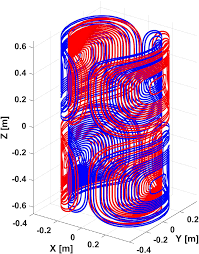
\includegraphics[height=5cm]{Bilddateien/GradientCoil.png}
            \caption{Schema einer Gradientenspule.}
        \end{figure}
    \end{Antwort}

\end{document}